\documentclass{article}

\usepackage{amsmath}
\usepackage{listings}
\usepackage{amsfonts}
\usepackage{amssymb}
\usepackage{graphicx}
\usepackage{titling}
\usepackage[utf8]{inputenc}
\usepackage[english]{babel}
\usepackage{amsmath}
\usepackage{fancyhdr}
\usepackage{lastpage}
\usepackage{textcomp}
\usepackage{graphicx}
\usepackage{hyperref}
\usepackage{float}

\addtolength{\oddsidemargin}{-.875in}
\addtolength{\evensidemargin}{-.875in}
\addtolength{\textwidth}{1.75in}
\addtolength{\topmargin}{-.875in}
\addtolength{\textheight}{1.75in}

\title{\Huge System Management \vspace{1cm}}
\author{Riccardo Biella, Elia Perrone, Nicolas Sala, Kevin Dominguez}
\date{Semestre primaverile 2019}
\setcounter{page}{0}
\pagestyle{fancy}
\fancyhf{}

\fancyfoot[C]{Page \thepage \hspace{1pt} of \pageref{LastPage}}


\begin{document}
\maketitle
\thispagestyle{empty}
\pagebreak

\section{Esercitazione 01}

\begin{figure}[H]
    \center
    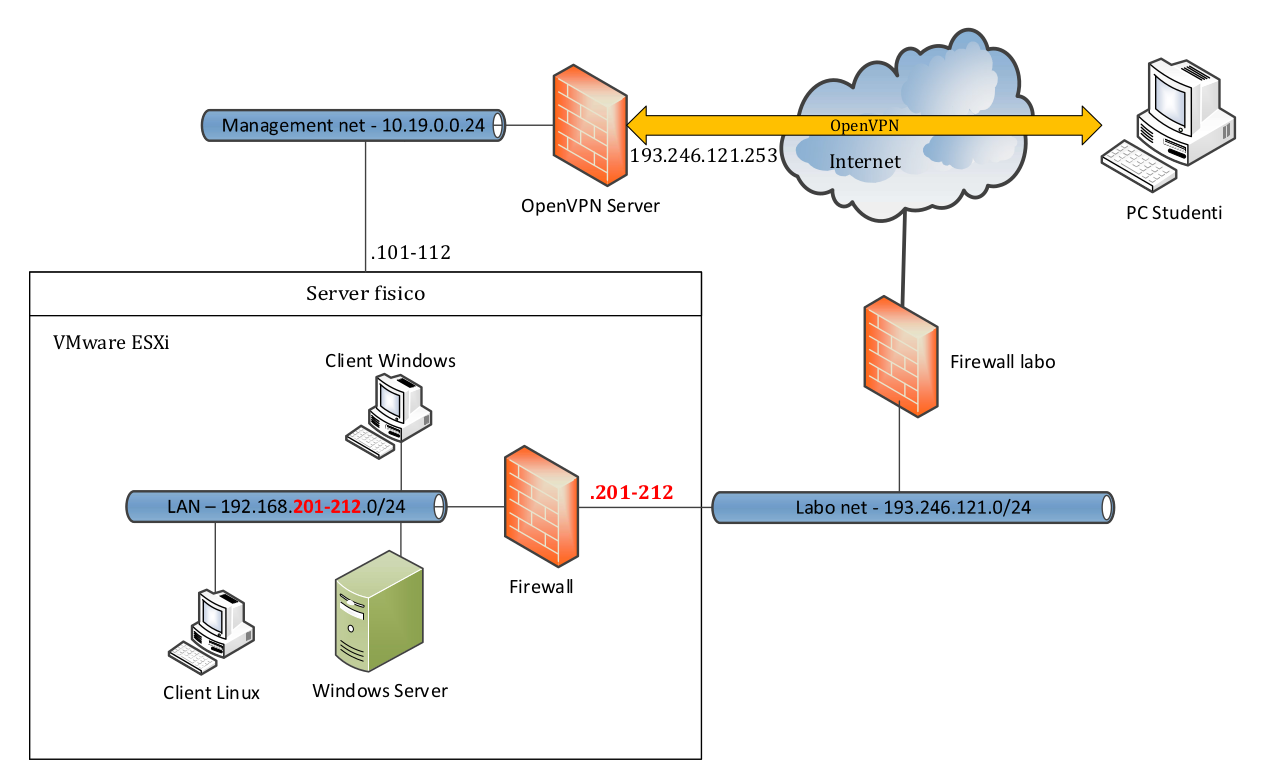
\includegraphics[scale=0.3]{images/schemaRete.png}
    \caption{Schema di rete base}\label{fig:1}
\end{figure}

\subsection{Specifiche del server utilizzato (Gateway GW2000h-GW170hq F1)}
Il server utilizzato per le esercitazioni può contenere fino a quattro nodi, con le seguenti caratteristiche:
\begin{figure}[H]
    \center
    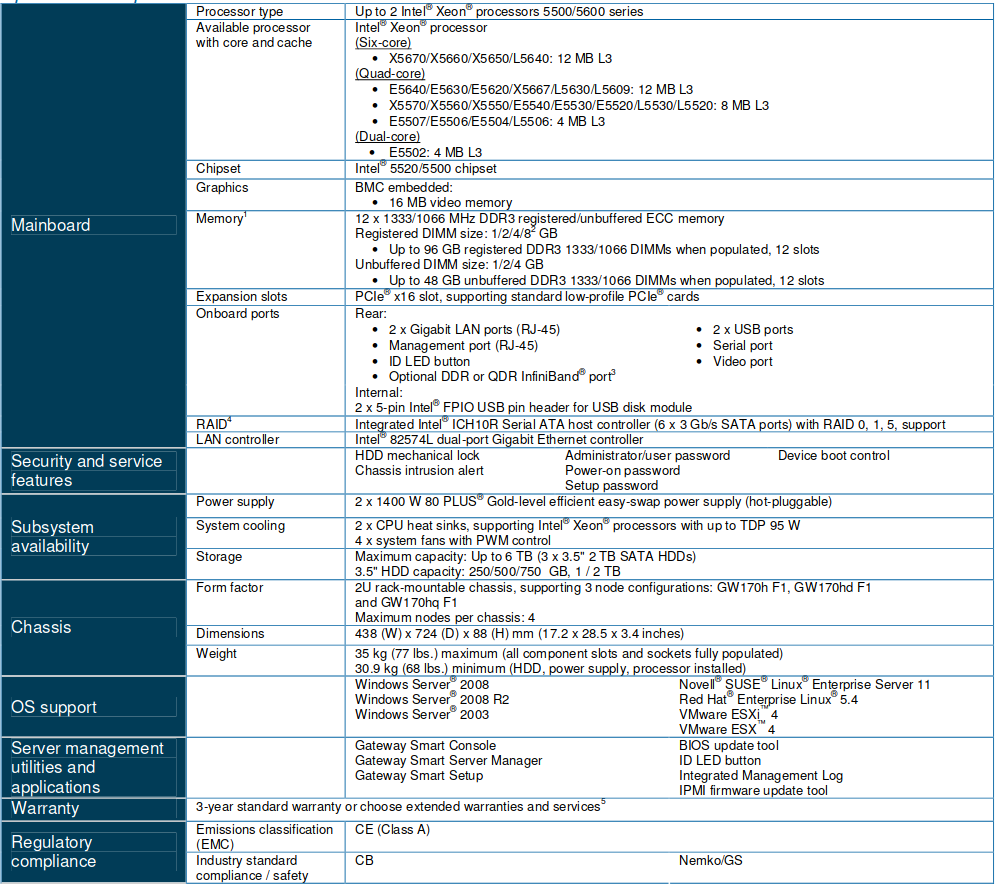
\includegraphics[scale=0.37]{images/specificheServer.png}
\end{figure}

\subsection{Hardware utilizzato}
Ad ogni gruppo è stata assegnata la gestione di un nodo all'interno del rack, esso dispone di un disco rigido, un SSD ed una periferica USB mediante il quale sarà possibile installare un hypervisor sul server.

\subsection{Interfaccia di gestione}ee
L'interfaccia di management del server, permette la gestione di numerosi aspetti della macchina, tra cui il controllo remoto, che utilizzaremo per lavorare sul server senza essere fisicamente presenti in laboratorio.
L'interfaccia di gestione è raggiungibile all'indirizzo IP: 10.19.0.106, a seguito di una connessione tramite client vpn, con le credenziali seguenti: \\  \textbf{username:} grp6 \\ \textbf{password:} System3m.Man\_grp6
\begin{figure}[H]
    \center
    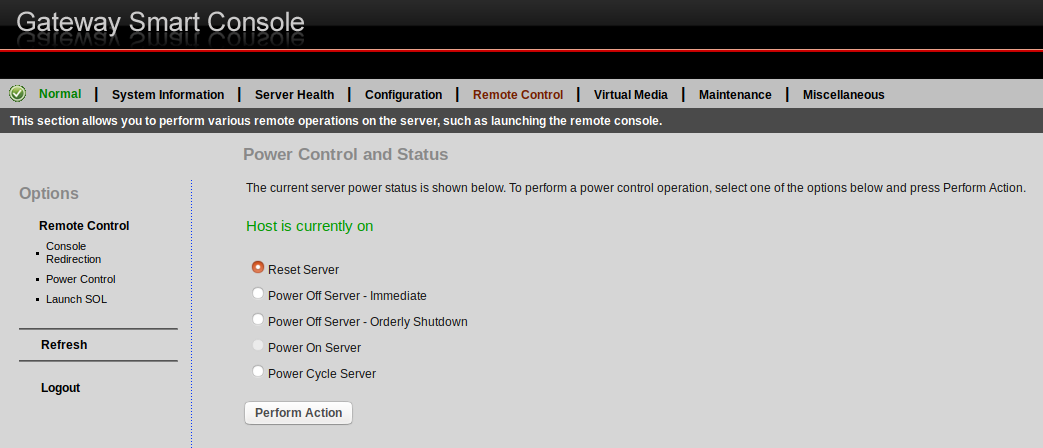
\includegraphics[scale=0.37]{images/GUIManagement.png}
\end{figure}

\subsection{OpenVPN}
\subsubsection{Obiettivo}
Connettersi tramite OpenVPN ed esplorare l’interfaccia di gestione del proprio
server (10.19.0.101-112) (user: root password: superuser) e documentare
azioni e informazioni disponibili.
(Gli account OpenVPN sono gestiti dal docente, che distribuisce ad ogni gruppo
un certificato personalizzato da importare nel proprio OpenVPN client – esempio
di nome di un certificato: SystemManagement-udp-1194-grp5.ovpn e
SystemManagement-udp-1194-grp5.p12).

\subsubsection{Installazione OpenVPN - Ubuntu x64}
\begin{enumerate}
    \item apt-get install openvpn \\ 
    Installiamo openvpn sulla nostra macchina
    \item openvpn --version \\
    Verifichiamo che l'installazione sia andata a buon fine
    \item openvpn --config client.ovpn \\
    Ci posizioniamo nella cartella (unzippata) che abbiamo scaricato da ICorsi,
    avviamo il client con il certificato corretto (.ovpn) che ci è stato fornito.
\end{enumerate}

\subsubsection{Problematiche} 
    Il server mette a disposizione una finestra con la quale è possibile lavorare in modalità
    grafica stile desktop remoto. Tale applicazione fa scaricare un file .JNLP dal server
    (lanciando il controllo renoto dalla console di gestione). Qualora il certificato di
    sicurezza fosse scaduto, si dovrà procedere a creare il trust al server nella macchina
    client (che altrimenti ne blocca l’esecuzione): aggiungere l’IP del server nelle Exception
    Site List di Java. Utilizzando OpenJDK non è possibile sfruttare l'interfaccia grafica di gestione, per questo 
    motivo abbiamo dovuto installare Oracle JRE.

\subsection{VMware ESXi}
\subsubsection{Descrizione}
VMware ESX Server è un prodotto per la virtualizzazione di livello enterprise offerto da VMware Inc., sussidiaria di Dell Technologies e ancor prima una divisione di EMC Corporation. ESX Server è un componente di un'offerta VMware più grande, VMware Infrastructure, che aggiunge servizi di amministrazione e di affidabilità al prodotto base. 
\subsubsection{Architettura}
Il server ESX include un microkernel che si interfaccia direttamente con la macchina. Nelle versioni ESX 3 e precedenti all'avvio viene lanciato un kernel Linux (una versione modificata di Red Hat Enterprise Linux) che analizza l'hardware della macchina e alcuni componenti di gestione, per poi cedere il controllo al componente vmkernel sviluppato di VMware. Questo è un microkernel con tre interfacce verso l'esterno:
\begin{enumerate}
    \item hardware
    \item sistema guest
    \item servizio console (servizio di gestione delle macchine virtuale che gira sul kernel che ha fatto partire vmkernel)
\end{enumerate}

\subsubsection{Installazione di VMWare} 
    Dopo esserci collegati all'interfaccia di gestione della macchina, sulla scheda abbiamo
    Remot Control abbiamo scaricato il file .JNLP ed attraverso la sua esecuzione
    abbiamo installato l'ipervisor: abbiamo settato un Ip statico pubblico in modo da non dover
    accedere ogni volta tramite VPN. Abbiamo utilizzato per installare VMWare una chiavete collegata direttamente al server.
    
\subsubsection{Altre opzioni di virtualizzazione}
\begin{enumerate}
    \item VirtualBox (Linux/Mac/Windows)
    \item Parallels (Linux/Mac/Windows)
    \item QEMU (Linux)
    \item Windows Virtual PC (Windows)

\end{enumerate}
\end{document}
